\renewcommand{\chaptername}{Componentes para la construcción de posicionador}
\chapter{Componentes para la construcción de posicionador} 
\markright{Componentes para la construcción de posicionador } 
\begin{center}
\begin{tcolorbox}[colback=gray!5!white, %Color del fondo
colframe=gray!75!black,
title= \center{\Large{resumen}} ]
En este capítulo se seleccionan cuales son los componentes necesarios para satisfacer los requerimientos de la sección \ref{req_sist}.   
\end{tcolorbox}
\end{center}    
\section{introducción}

En este capítulo, se van a mostrar cuales son los componentes, que debe tener el sistema en su versión final. Estos componentes se basan en los requerimientos definidos en la sección \ref{req_sist}. En el mismo, se ha divido en dos tipos de requerimientos: Funcionales y de sistema. 

\section{Componentes del Proyecto}

La interconexión de las partes dentro de la institución debe responder al siguiente diagrama del sistema general: 
%---------------- diagrama en bloques -----------------------% 
\begin{figure}[ht]	
	\centering
	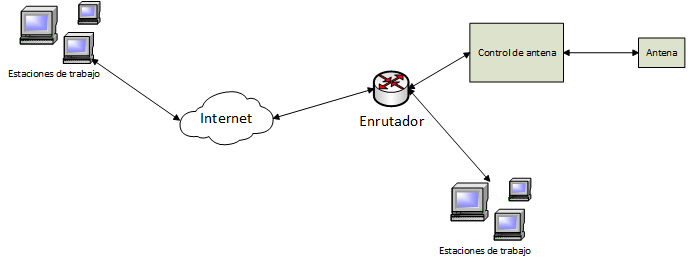
\includegraphics[scale=0.8]{parte_1/cap2/ssgen}
	\caption{Diagrama del sistema general}
	\label{fig:fig_ssgen}
\end{figure}


Donde el bloque desarrollado en la presente tesis es el control de antena de la figura \ref{fig:fig_ssgen},y la configuración de software sobre las estaciones de trabajo dentro de la institución. 

Por lo expuesto en la sección \ref{req_sist}(requisitos del sistema), el sistema que debe realizar el control de la posición sobre la antena debe tener los siguientes componentes: 

\begin{enumerate}
	\item Microcontrolador o computadora para realizar el movimiento de la antena, además debe responder a una PC y realizar el movimiento de la antena.    
	\item Interfaz de usuario con el estado del sistema(interfaz electrónica o pantalla para mostrar el estado del sistema).
	\item Interfaz de red, cableada para poder recibir ordenes desde una PC dentro de la institución. 
	\item Mediciones angulares en ambos ejes de la antena.  
	\item Sistemas electrónicos para manejo de motores. 
	\item Software PC de seguimiento de satélites que cuente con conectividad a la red.  
\end{enumerate}

Estos items, cumplen todos los requerimientos, tanto funcionales como de sistema. La escalabilidad y la independencia  se realiza mediante el microcontrolador, ya qué, se puede actualizar el software sobre el mismo, logrando que el mismo sea escalable. La autocalibración, 
control, y el seguimiento de satélites, naturales o artificiales, y estrellas, se consigue con la combinación del microcontrolador con los sistemas electrónicos de manejo de motores. La recepción desde una PC de los datos, se realiza mediante la interfaz de red. Ambos requerimientos(funcionales y de sistema), deben realizarse mediante la programación del microcontrolador, y la construcción del sistema electrónico de manejo de los motores. Cabe destacar, que se deben realizar dos sistemas electrónicos para el manejo de los motores, ya que el mismo, tiene dos motores, independientes entre si, el cual genera movimientos independientes de la antena. El requisito de bajo costo y disponibilidad en el mercado local, se analiza en el siguiente capítulo. 


%
%Estas características, para ser cumplidas, requieren que el sistema de control de la antena, tenga una cierta inteligencia para realizar las tareas de manera simultanea. Esto conlleva a que el sistema debe poseer una computadora o microcontrolador capaz de realizar todas estas tareas, además, debe requerir hardware adicional, para interactuar con los motores, y debe requerir algún mecanismo de medición de posición, para poder realizar un lazo de control realimentado. 
%Esto conlleva al siguiente diagrama en bloques, que es el control de antena,de la figura \ref{fig:fig_ssgen} visto con mayor detalles: 
%%\vspace{length}
%
%\begin{figure}[H]
%	\raggedleft
%	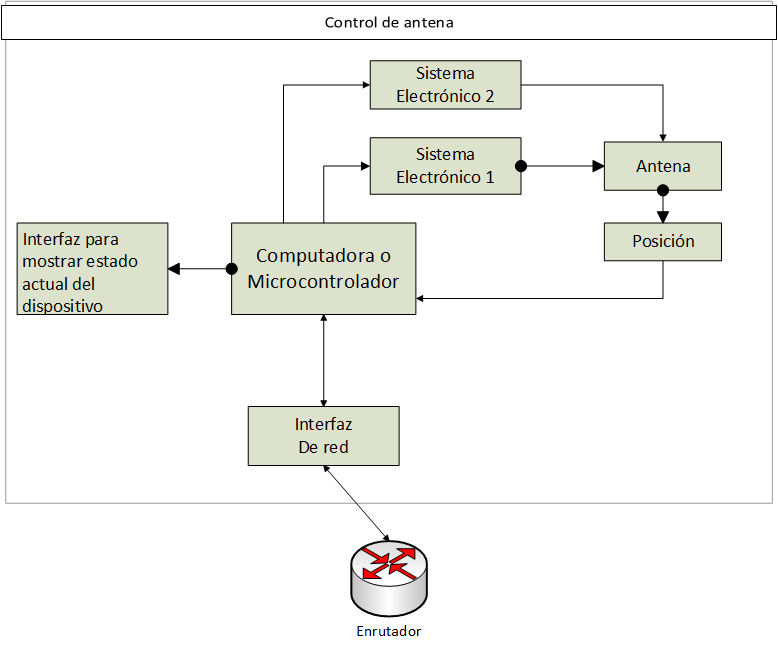
\includegraphics[width= 1.0\textwidth,height=8.6cm]{parte_1/cap2/scontrol} 
%	\vspace{-0.6cm}	
%	\caption{Diagrama del sistema de control}
%	\label{fig_sistema_solucion}
%\end{figure}
%
%En la figura anterior, se tienen dos sistemas electrónicos de posición,ya que la mecánica existente sobre la antena(ver figura \ref{fig_mec_ant} ) permite la independencia de movimientos.  




